\chapter{Estado de la técnica}
\section{Trazabilidad de tiempo}
\subsection{Global Navigation Satellite System (GNSS)}
La GNSS se trata de un conjunto de satélites que permiten a un usuario situado en La Tierra calcular su posición exacta de manera bastante precisas (desde algunos metros hasta centímetros de precisión). Existen varios de estos sistemas de posicionamiento, entre ellos están GPS, GLONASS, Galileo, etc. Este tipo de sistemas consisten en una constelación de satélites encargados de transmitir unas determinadas señales sobre La Tierra. Los relojes que portan dichos satélites están sincronizados en base a una escala temporal definida por el sistema propio de cada constelación. Con esto se consigue que las señales emitidas por cada satélite compartan una misma referencia temporal. Esto es vital para el buen funcionamiento del sistema. \newline

El equipo receptor de un usuario que pretende usar el sistema GNSS para determinar su posición consiste de una antena que recibe las señales emitidas por estos satélites, y un dispositivo que sea capaz de traducir estas señales recibidas en una posición. Los cálculos realizados por este dispositivo se basan en la diferencia temporal entre la emisión de la señal por parte de los satélites y la recepción por parte de la antena del usuario. Este retardo de propagación se traduce fácilmente en una distancia que separa a cada satélite de la antena, ya que la señal viaja a la velocidad de la luz. \newline

La distancia entre un satélite y la antena no da la posición exacta de la antena, sólo informa de una esfera alrededor del satélite en la que debe encontrarse la antena. Para calcular la posición exacta se necesitan varias de estas medidas de diferentes satélites. Conociendo la distancia a la que se encuentra la antena respecto a dos satélites distintos se traduce en dos esferas distintas sobre las cuales debe localizarse la antena. Es evidente que la antena se encuentra en la intersección de estas dos esferas, que como se observa en la figura XXXXXXXx es un círculo.

\begin{figure}
	\centering
	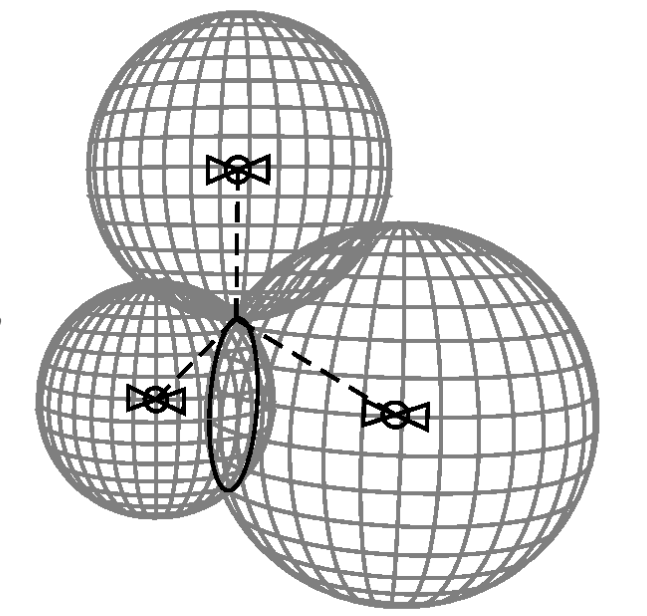
\includegraphics[width=1\textwidth]{imagenes/interseccion2esferas.PNG}
	\caption{\label{fig1}Intersección de las 2 esferas creadas por satélites \cite{gnss}.}
\end{figure}

La intersección de este círculo con una tercera esfera (relacionada con la distancia respecto de un satélite a la que se encuentra la antena) reducirá a 2 los posibles puntos en los que se encuentra la antena. Una cuarta esfera será necesaria para decidir cuál de esos dos puntos se corresponde con la correcta localización de la antena. \newline\\

La situación descrita en la figura XXXXXXXXXXXX en la que los satélites se distribuyen espacialmente alrededor del receptor es demasiado optimista. El receptor presumiblemente se situará en la superficie terrestre, por lo que solamente tendrá visibles los satélites que se encuentren sobre él. Es necesario por tanto usar la técnica observada en la figura XXXXXXXXXXXXX. \newline

\begin{figure}
	\centering
	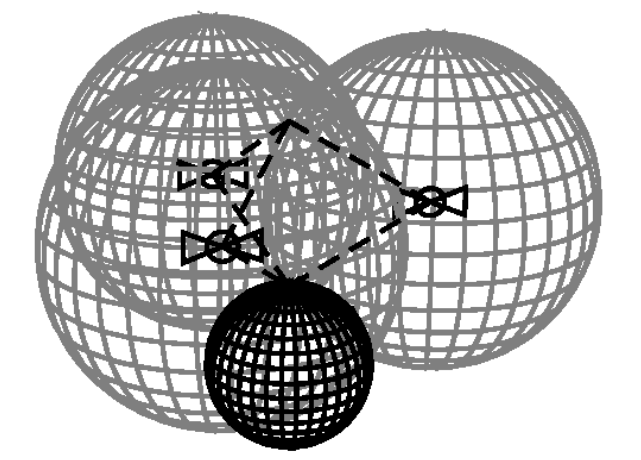
\includegraphics[width=1\textwidth]{imagenes/tierra4esfera.PNG}
	\caption{\label{fig1}La Tierra hace de cuarta esfera \cite{gnss}.}
\end{figure}

En esta situación, se tiene la intersección formada por las esferas de 3 satélites, y será la superficie de La Tierra la encargada de decidir cuál de los dos puntos de esa intersección es el correcto. La metodología es similar a la anterior, con la única diferencia de la cuarta esfera. \newline

La descripción del funcionamiento dada del sistema GNSS se corresponde con una situación idílica, que en realidad no se corresponde con lo que ocurre en el mundo real. Existen varios problemas para los cuales se ha tenido que adaptar la metodología seguida para calcular la posición de la antena receptora. \newline

Para poder calcular el retardo de propagación de la señal enviada por el satélite, esta va sellada con el tiempo en el que se emitió. Esto implica que el receptor debe tener un reloj preciso y sincronizado con la referencia temporal de los satélites. Esta implicación no es realista, por lo que se producen pequeños errores temporales, que a la velocidad de la luz se traducen en grandes errores en la localización. Estos errores pueden llegar a hacer que las 4 esferas no se corten en un único punto común, por lo que son insostenibles. La solución consiste en una constante corrección del reloj del receptor que haga a las 4 esferas coincidir en un único punto. \newline

Otro de los inconvenientes deriva del cálculo de los centros de estas esferas utilizadas para el cálculo de la localización de la antena. Esto implica que cada satélite debe ser capaz de calcular su posición exacta en el espacio, cosa que no sucede. Los satélites no son capaces de calcular su posición exactamente, lo que de nuevo se traducirá en que las 4 esferas no se corten en un único punto. Para solventar este inconveniente se sigue una estrategia distinta a la anterior. Se usarán los cálculos de tantos satélites como sea posible medir para calcular la posición de la antena de la manera más exacta posible. \newline

Suponiendo que los anteriores problemas quedan solucionados, para que la medida de la posición sea precisa se necesitará que la señal viaje en el vacío. El retardo de propagación se ha supuesto para que el medio de transmisión sea el vacío, cosa que en el mundo real no será así. La señal atravesará algunas capas como la ionosfera y la troposfera. En estas capas de la atmósfera la velocidad será inferior a la velocidad de la luz. Se estudia como afectan las velocidades de propagación en estos medios y se realizan las correcciones pertinentes para solventar este problema. \newline


\subsection{Transferencia de tiempo}

Cada sistema GNSS tiene su propia referencia temporal necesaria para calcular el comportamiento de los relojes contenidos en los satélites de la constelación. Esta referencia temporal es transmitida por dichos satélites en sus datos de navegación. Esta información se corresponde con la diferencia de la hora del reloj del satélite y la hora UTC. Surge entonces el concepto de transferencia o trazabilidad de tiempo consistente en la comparación de dos relojes remotos que han sido conectados a receptores GNSS. Si se conoce la localización del satélite y de la estación receptora, se puede deducir el error de sincronización con respecto a la referencia temporal del sistema GNSS. A su vez se pueden deducir diferencias temporales del reloj de diferentes laboratorios o estaciones. El funcionamiento básico del sistema usado para comparar dos relojes es el observado en la figura XXXXXXXXXXxx.\newline

\begin{figure}
	\centering
	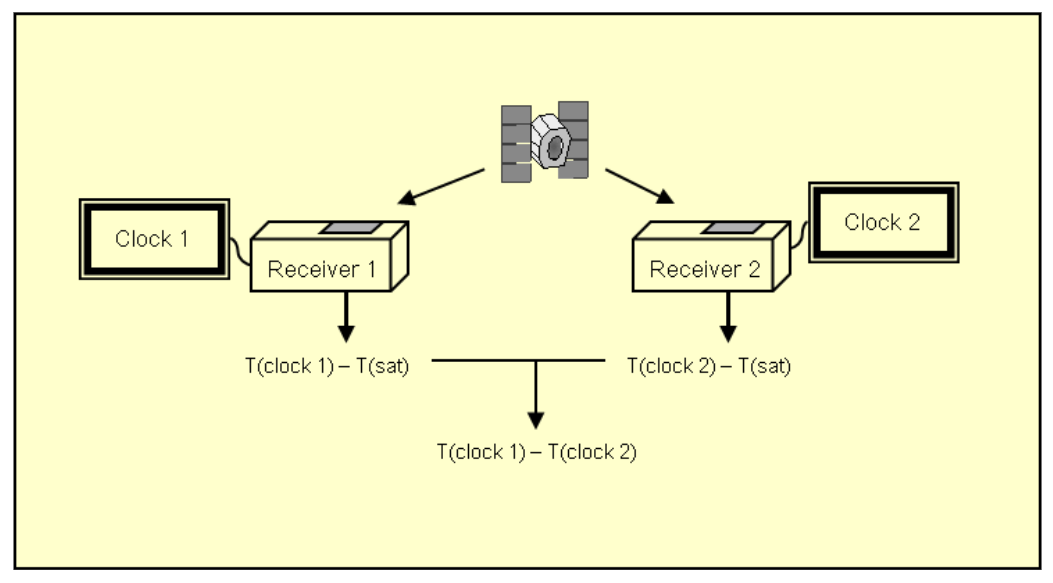
\includegraphics[width=1\textwidth]{imagenes/2clockscompare.PNG}
	\caption{\label{fig1}Escenario básico para la comparación de 2 relojes \cite{gnss}.}
\end{figure}

La figura XXXXXX representa una situación simplificada en la que se hace uso de un único satélite. Sin embargo, existen dos técnicas distintas en las que se hace uso de más de un satélite, que son las que realmente se llevan a cabo.

\subsubsection{Satélites en Common View (CV)}
Esta técnica hace uso de los satélites que son comunes durante un determinado tiempo para los dos relojes que se quieren comparar. Al ser satélites comunes se puede obtener la diferencia entre el reloj 1 y el reloj 2 en base a las medidas tomadas de cada satélite. El siguiente paso será combinar las comparaciones obtenidas con cada satélite para obtener la media del error de sincronización entre relojes. La figura XXXXXXXXXx representa la situación que se tendría al hacer uso de esta técnica.\newline

\begin{figure}
	\centering
	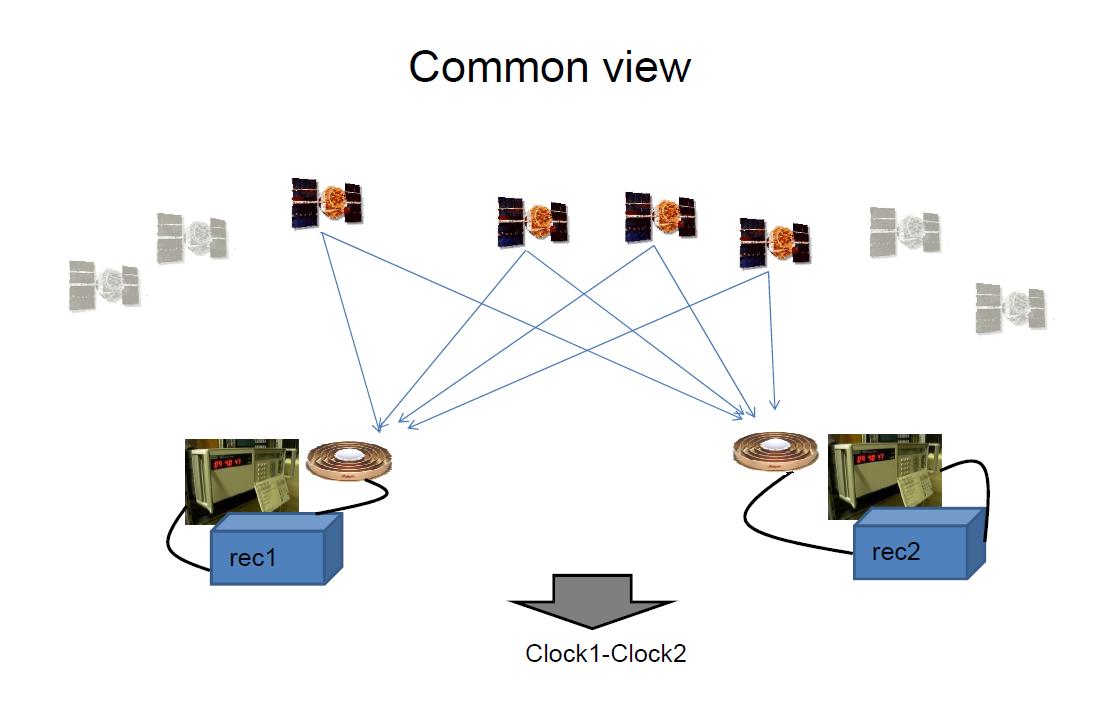
\includegraphics[width=1\textwidth]{imagenes/commonview.PNG}
	\caption{\label{fig1}Escenario con satélites en Common View \cite{timetransfer}.}
\end{figure}

\subsubsection{Satélites All in view (AV)}
Otra de las técnicas usada para la trazabilidad del tiempo consiste en obtener el error de sincronización respecto a la referencia temporal usada por el sistema. En este caso la referencia temporal será la hora UTC. Se hará uso de las medidas tomadas de cada satélite visto por el receptor. En los datos de navegación cada satélite transmitirá la información relacionada con el error de sincronización entre el reloj del satélite respecto a la referencia temporal del sistema. Por lo tanto, del error de sincronización entre el reloj del receptor y el del satélite se podrá deducir el error de sincronización existente entre el reloj del receptor y la referencia temporal del sistema. Cada reloj tomará estas medidas de todos los satélites que tenga a la vista como se observa en la figura XXXXXXXXXXX. Se obtiene así la media del error de sincronización de cada reloj con la referencia temporal del sistema. Como esta referencia temporal es común para todo el sistema, los dos relojes se estarán comparando con la misma referencia. De esto se podrá deducir fácilmente la comparación entre el reloj 1 y el reloj 2.\newline

\begin{figure}
	\centering
	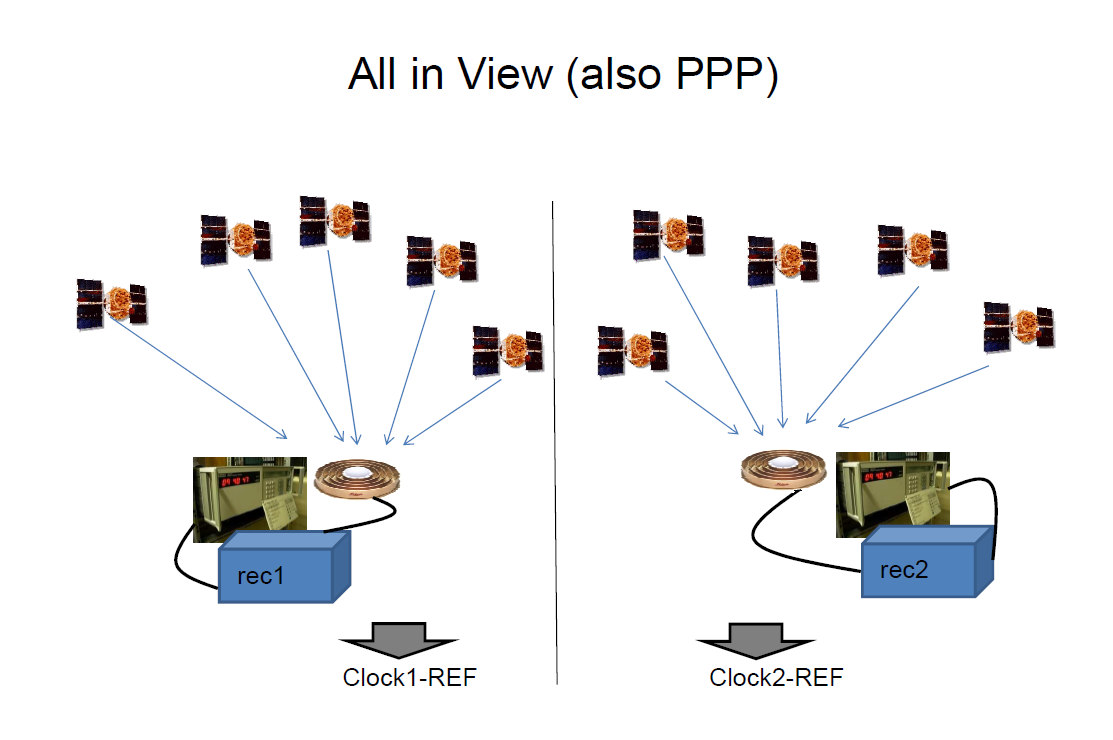
\includegraphics[width=1\textwidth]{imagenes/allinview.PNG}
	\caption{\label{fig1}Escenario con satélites All in View \cite{timetransfer}.}
\end{figure}

El uso de una u otra técnica dependerá principalmente de los satélites de los que se disponga. El resultado obtenido será en ambos casos el mismo, con la diferencia de la precisión. El uso de métodos como Precise Point Positioning (PPP) será uno de los principales factores determinantes para la precisión de los resultados obtenidos.\newline

\subsection{R2CGGTTS}
El uso de la transferencia de tiempo ha sido muy extendido desde los años 80. El Bureau International des Poids et Mesures (BIPM) lo lleva utilizando desde entonces para comparar las realizaciones del tiempo UTC por parte de los laboratorios de tiempo, con el objetivo de generar el International Atomic Time (TAI). Otro de los usos más extendido consiste en el uso de la transferencia de tiempo para sincronizar relojes locales con las referencias legales de tiempo situadas en los Institutos Nacionales de Meteorología. Se hizo necesario crear un estándar con el que formatear los resultados obtenidos de la transferencia de tiempo para facilitar su uso. El estándar fue conocido como Common GPS GLONASS Time Transfer Standard (CGGTTS). \newline

Los ficheros CGGTTS pueden ser directamente producidos por el receptor GNSS. También podrán ser reconstruidos a partir de las medidas y los datos de navegación proporcionadas por el receptor en forma de fichero RINEX (Receiver INdependent EXchange). Para realizar esta tarea el Royal Observatory of Belgium (ROB) ha creado una herramienta capaz de crear ficheros CGGTTS a partir de los ficheros RINEX. Este software, denominado R2CGGTTS, es distribuido públicamente a través del servidor FTP del BIPM. \newline

Los datos relacionados con los errores de sincronización aparecen en las dos columnas indicadas en la figura XXXXXXXXXXXXx.\newline

\begin{figure}[H]
	\centering
	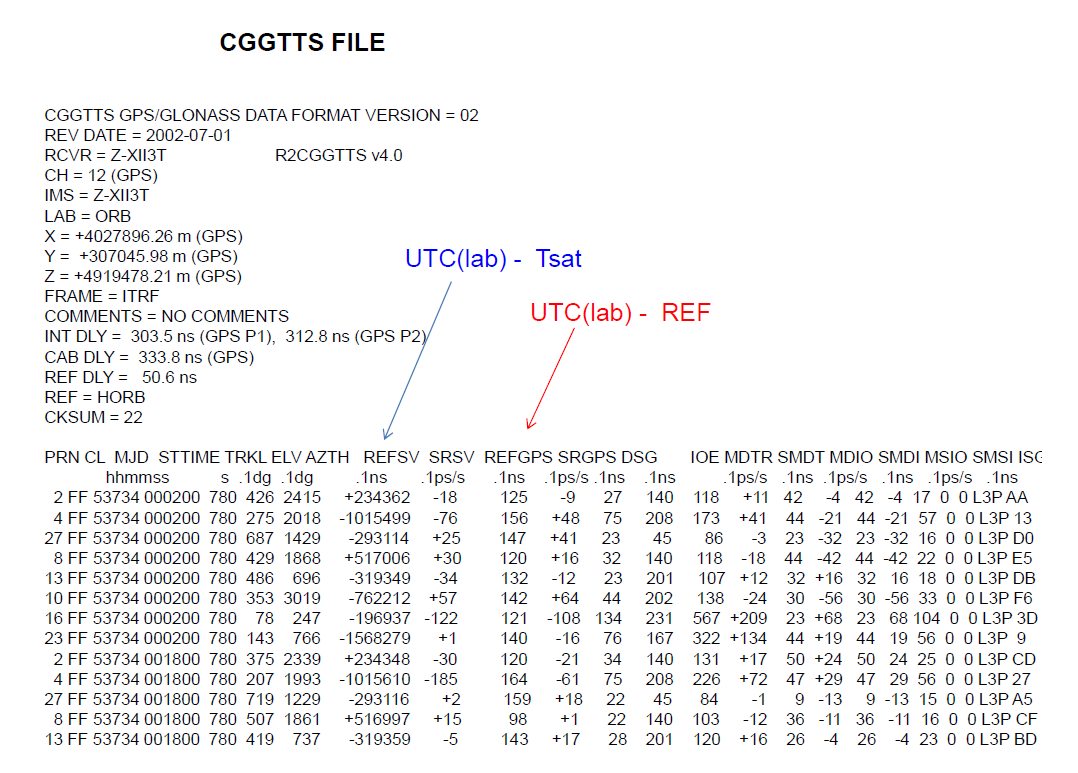
\includegraphics[width=1\textwidth]{imagenes/cggtts.PNG}
	\caption{\label{fig1}Ejemplo de fichero CGGTTS \cite{timetransfer}.}
\end{figure}



\section{Revisión de tecnologías Blockchain}

En el apartado de Introducción se ha dado una visión muy general de cómo surgió blockchain y de sus hitos más importantes. La explicación de las redes blockchain ha sido tan simple como ha sido posible para entender la motivación y los objetivos del proyecto. Sin embargo, es necesario conocer con más detalle el funcionamiento y las posibilidades que ofrecen los distintos tipos de redes blockchain para la correcta comprensión del trabajo. Notar que, pese a que la explicación se realizará en base a la blockchain de Bitcoin, la explicación es extensible a la gran mayoría de redes blockchain.\newline

\subsection{Criptografía}

La criptografía pese a ser prácticamente transparente para el usuario, juega un papel fundamental en la actualidad. Acciones tan cotidianas como enviar un correo electrónico o pagar con tarjeta de crédito funcionan gracias a la criptografía. La criptografía aporta seguridad a estos procedimientos. ¿Por qué se confía en la criptografía? La criptografía se basa en una ciencia exacta, como son las matemáticas, y en algoritmos muy estudiados por la comunidad científica. Varios de estos algoritmos de la criptografía son usados en la tecnología blockchain para aportar seguridad. Son esenciales para su correcto funcionamiento.\newline

\subsubsection{Las funciones Hash}
La traducción al castellano de blockchain es cadena de bloques. En este apartado se explica la metodología que se sigue para que los bloques de información queden encadenados y cuál es el objetivo de esto.
Una función hash es una función unidireccional. Las funciones unidireccionales se definen como:\newline


XXXXXXx f:X -- Y,f(x)=y \\
La principal característica de estas funciones es que f(x) es fácil de calcular, pero calcular fXXXX(-1) (y) es computacionalmente irrealizable. Apoyadas en esta característica, las funciones hash se aplican sobre mensajes M para proporcionar un resumen del mismo denominado m. El resumen m tendrá una longitud fija independiente de la longitud del mensaje M.
Existen numerosas funciones hash. Sin embargo, para que una función hash se considere segura y pueda ser utilizada en criptografía debe cumplir una serie de requisitos:

\begin{enumerate}
	\item 1.	Dependencia de bits: se corresponde con la propiedad de dispersión de las funciones hash. El resumen debe depender de todos los bits del mensaje. Esto significa que, si se cambia un bit del mensaje, cambian de media la mitad de los bits del resumen.
	\item 2.	Resistencia a la preimagen: dado un resumen m, debe ser computacionalmente difícil obtener M de modo que H(M) = m.
	\item 3.	Resistencia a la segunda preimagen: dado un mensaje M, debe ser computacionalmente difícil encontrar otro mensaje N cuyos resúmenes coincidan, es decir H(M) = H(N).
	\item 4.	Resistencia a colisiones: debe ser computacionalmente difícil encontrar una colisión. Una colisión consiste en dos mensajes M y N cuyos resúmenes coincidan. 
\end{enumerate}

En definitiva, las funciones hash permiten obtener un identificador único de un mensaje. Identificador a partir del cual no se podrá obtener el mensaje original y que garantiza la integridad del mismo. Este aspecto es lo que hace a las funciones hash indispensables para blockchain.

\paragraph{Aplicación de las funciones Hash a Blockchain}
Una cadena de bloques se origina a partir de un primer bloque, el bloque génesis. Se pretende que todos los bloques que se vayan añadiendo a la cadena estén enlazados de alguna manera inequívoca con todos los bloques previos hasta llegar al génesis. Esto se consigue con las funciones hash siguiendo la siguiente metodología desde el bloque génesis:

\begin{enumerate}
	\item 1.	Haciendo uso de una función hash, se obtiene el resumen o hash del bloque génesis. El hash será un código de longitud fija que identifica inequívocamente al bloque génesis.
	\item 2.	Para crear el siguiente bloque de la cadena, se incluye en este un campo que contendrá el hash del bloque anterior.
	\item 3.	Una vez finalizada la creación del nuevo bloque, se le calcula el hash al nuevo bloque y se vuelve al paso 2.
\end{enumerate}

Con este procedimiento se consigue que el hash de un bloque N de la cadena identifique inequívocamente a toda la cadena de bloques desde el bloque génesis hasta el bloque N. Se garantiza que toda la cadena de bloques permanece íntegra y que si alguno de los bloques sufre algún cambio se alterarán los hashes de todos los bloques posteriores. El resultado partiendo desde el bloque génesis se observa en la figura XXXXXXXXXXXXxxx.\newline

\begin{figure}
	\centering
	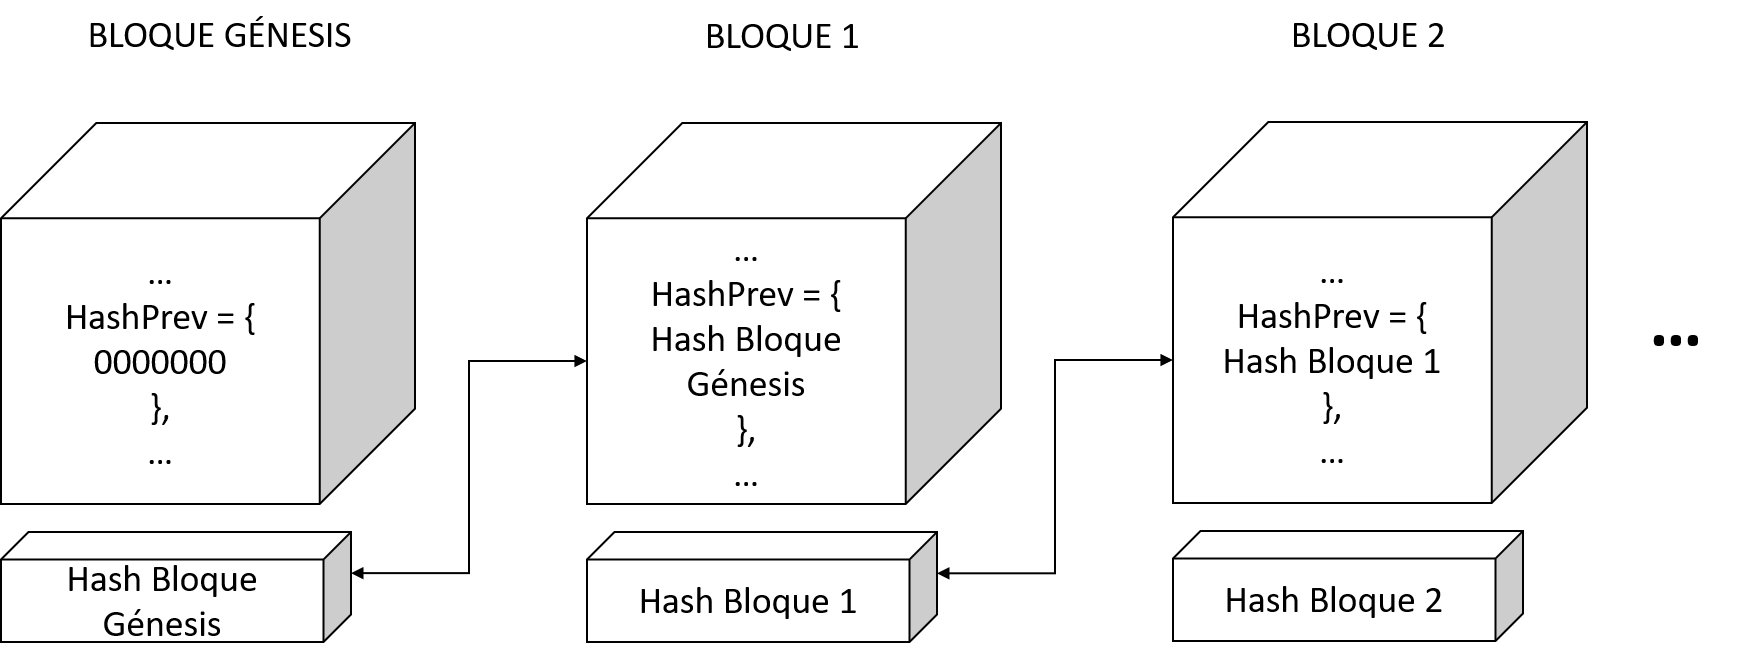
\includegraphics[width=1\textwidth]{imagenes/PrevHashes.PNG}
	\caption{\label{fig1}Estructura de hashes de Blockchain. XXX}
\end{figure}

\subsubsection{Criptografía de clave asimétrica}
En 1976 Diffie y Hellman proponen un nuevo método para la distribución de claves. El propósito de este método era permitir a dos extremos de una comunicación establecer una clave simétrica sin que estos hayan tenido un contacto previo o usen un canal seguro. Esta propuesta daba solución al intercambio de claves simétricas, pero no permitía el cifrado. Sin embargo, este método dio origen un año después al primer algoritmo de cifrado de clave asimétrica. En 1977 nace el algoritmo RSA de la mano de Rivest, Shamir y Adleman. Este es uno de los algoritmos más utilizados incluso a día de hoy. RSA permite no sólo el cifrado sino también la firma digital. \newline

La principal innovación que introduce este tipo de criptografía es el uso de un par de claves. Se tendrá una clave pública y una clave privada. Como su propio nombre indica, la clave pública será conocida por todos, en cambio la clave privada sólo la debe conocer su propietario. De esta manera deja de ser necesario el intercambio de una clave simétrica a través de un canal seguro.
La criptografía asimétrica se apoya en tres tipos de problemas matemáticos:

\begin{enumerate}
	\item Problema de la factorización de enteros
	\item Logaritmo discreto
	\item Curvas elípticas
\end{enumerate}

Al igual que ocurría con las funciones hash, las funciones matemáticas escogidas para estos problemas tienen como principal característica el fácil cálculo en un sentido, pero muy difícil computacionalmente en el sentido inverso. De nuevo se trata de funciones unidireccionales. \newline

El cifrado de un mensaje mediante criptografía de clave simétrica sigue el siguiente esquema:

\begin{enumerate}
	\item El emisor obtiene la clave pública del destinatario por cualquier canal (puede ser inseguro).
	\item El emisor cifra el mensaje con la clave pública del destinatario.
	\item El emisor envía el mensaje cifrado a través de cualquier canal ya que solamente el poseedor de la clave privada asociada a la clave pública con la que se cifró el mensaje podrá descifrarlo. En este caso el destinatario.
	\item El destinatario recibe el mensaje cifrado y haciendo uso de su clave privada obtiene el mensaje en texto plano.
\end{enumerate}

Este esquema explica un simple intercambio de un mensaje cifrado. Sin embargo, la criptografía de clave asimétrica abre un abanico de posibilidades a protocolos más complicados que ofrezcan distintas cosas. Un claro ejemplo es la firma digital. La tecnología blockchain también hace uso de este tipo de cifrado. \newline

Los principales aportes que hacen al cifrado asimétrico tan interesante para blockchain son:

\begin{enumerate}
	\item No repudio. Si un usuario firma un mensaje con su clave privada, no podrá negar haberlo hecho.
	\item Identificación. Ambos extremos de una comunicación quedan identificados.
\end{enumerate}

\paragraph{Aplicación de la criptografía a Blockchain}

Este apartado describe el uso que la tecnología blockchain hace de la criptografía de clave asimétrica. Una red blockchain es una red P2P distribuida, por lo tanto, ninguno de los usuarios es a priori conocido o fiable. Dentro de esta red la identidad de los usuarios es pseudoanónima. No se conoce la identidad real de los usuarios, pero tampoco es necesario. Solamente es necesario un identificador único que los identifique dentro de la red. Cada usuario tiene un par de claves asimétricas (pública y privada). Este identificador único se corresponde con la clave pública del usuario (existe un proceso que transforma la clave pública en una dirección, pero no es relevante). \newline

La mejor forma de observar el uso que se hace de este par de claves es describir los pasos que se siguen para realizar una transacción en la blockchain de Bitcoin.

\begin{enumerate}
	\item El receptor envía su clave pública al emisor de la transacción.
	\item El emisor incluye en el campo destinatario de la transacción la clave pública del destinatario.
	\item La transacción, entre otros datos, incluye la cantidad de bitcoins a transferir.
	\item El emisor cifra la transacción con su clave privada. En este paso el emisor está demostrando que posee una cierta cantidad de bitcoins y acepta que ahora pasan a ser propiedad del destinatario.
	\item La transacción se transmitirá a todos los usuarios de la red que la validarán e incluirán en la blockchain.
\end{enumerate}

El paso 4 resulta crucial ya que de él se obtiene la identificación y el no repudio de la transacción. Resulta evidente que la criptografía de clave asimétrica es idónea y totalmente necesaria para el correcto funcionamiento de cualquier red blockchain.

\section{Teoría de juegos}
La teoría de juegos es una rama de las matemáticas aplicada que analiza la toma de decisiones en situaciones en las que la decisión no sólo se basa en el punto de vista de un jugador, sino teniendo en cuenta las decisiones tomadas por el resto de jugadores. Se entiende por juego una situación en la que un jugador podrá obtener recompensas o perjuicios según la decisión que hayan tomado él mismo y el resto de jugadores. \newline

El concepto relacionado con la teoría de juegos más importante para blockchain es el equilibrio de Nash. Este concepto, creado por John Nash, afirma que, si todos los jugadores siguen una estrategia óptima, ningún jugador saldrá beneficiado si cambia individualmente su estrategia. El equilibrio de Nash está directamente relacionado con la expresión “Si la mayoría de los usuarios de la red actúa correctamente la blockchain funcionará correctamente”. Ciertos usuarios de la red podrían intentar hacer trampa incluyendo bloques a la cadena sin resolver la prueba de trabajo, incluir transacciones inválidas, etc. Sin embargo, blockchain está diseñada para que se mantenga el equilibrio de Nash. Si se incluye un bloque válido encima de uno inválido, este pasa automáticamente a ser inválido también. Por lo tanto, la estrategia que les interesa a los usuarios es actuar de manera correcta y elegir la situación más estable. Se mantendrá el equilibrio de Nash mientras la mayoría de los usuarios actúen de manera honesta. Si usuarios con más de la mitad del poder computacional de la red deciden actuar de manera deshonesta, el equilibrio de Nash pasará a localizarse del lado de los usuarios deshonestos y la blockchain pasará a estar corrompida. Esta es la explicación del famoso ataque del 51\%.

\section{Aspectos clave del protocolo Blockchain}
\subsection{Concepto de minado}
Hasta este apartado se había descrito la red blockchain como una red P2P formada por usuarios. Se utiliza el termino usuario por simplicidad. En este apartado se explica en qué consiste la minería de bloques en blockchain y quienes son los que la realizan. \newline

En realidad, la red blockchain la componen una serie de nodos denominados mineros. Los usuarios simplemente son los encargados de enviar sus propias transacciones a la red cuando lo deseen. La tarea de los mineros consiste en minar bloques que contengan transacciones con el objetivo de obtener una recompensa. Minar un bloque es como se denomina al acto de resolver la prueba de trabajo descrita de manera simplificada en el APARTADO XXXXXXXXXXXXXxxX.

\subsubsection{Prueba de trabajo}
En el apartado XXXXXXXXxx se describe la prueba de trabajo como un problema de solución muy compleja, pero de verificación muy sencilla. Existen multitud de problemas matemáticos que se podrían utilizar para la prueba de trabajo de blockchain. El problema elegido para blockchain es el cálculo de un resumen hash con una característica determinada. El hash que sirva de solución a la prueba de trabajo de un bloque debe tener una determinada cantidad de ceros (‘000…’) al principio. La cantidad de ceros estará determinada por la dificultad, que a su vez está marcada por la cantidad de poder computacional total de la red. El resumen hash se calcula al bloque que se pretende incluir en cadena de bloques.
Por lo tanto, los pasos que deberá seguir un minero que pretende resolver la prueba de trabajo y minar un nuevo bloque son los siguientes:
\begin{enumerate}
	\item Calcular la dificultad del siguiente bloque de la cadena. Esta dificultad se calcula en base a una expresión que depende del tiempo que se ha tardado en minar los últimos bloques de la cadena. La dificultad determina el número de ceros que debe tener el hash del siguiente bloque a incluir en la cadena.
	\item Construir un bloque válido que pretenda incluir en la cadena.
	\item Dentro del bloque existe un campo denominado nonce que será variable y que no aporta ninguna información. El minero deberá ir cambiando el campo nonce hasta que obtenga un hash del bloque que tenga el número de ceros que satisfaga la prueba de trabajo.
	\item Dar un valor al campo nonce.
	\item Calcular el hash del bloque con el nonce incluido en el punto 4.
	\item Si el hash obtenido no satisface la prueba de trabajo, volver al punto 4. En caso de que el hash satisfaga la prueba de trabajo, se dice que se ha minado el bloque. El minero puede proceder a difundir este bloque minado para que los demás lo validen e incluyan a la cadena de bloques. El hecho de incluir el bloque en la cadena significa que cuando el resto de mineros vuelvan a realizar este algoritmo, en el paso 2 incluyan el hash del bloque recién minado en el campo hash previo. Así este permanecerá en la cadena inalterable para siempre.
\end{enumerate}

Este es el algoritmo que deberá seguir todo minero para minar un nuevo bloque. Notar que es en los puntos 4, 5 y 6 donde se emplea la gran parte del poder de cómputo para el minado.

\subsubsection{Creación de un bloque válido}
En el algoritmo que debe seguir un minero para minar un nuevo bloque se observa que el segundo paso es crear un nuevo bloque válido a incluir en la cadena. Para entender en qué consiste este paso en detalle es necesario saber de qué está compuesto un bloque.\newline 

\begin{figure}
	\centering
	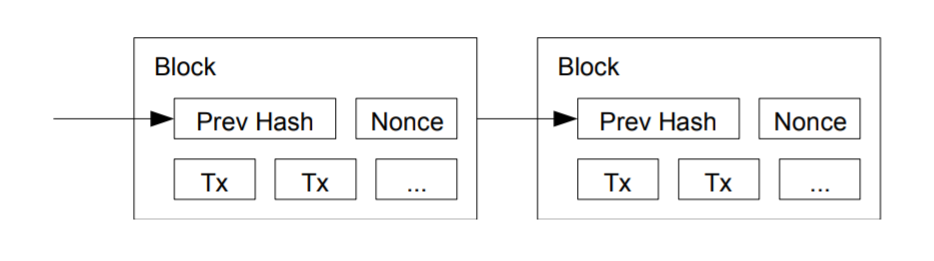
\includegraphics[width=1\textwidth]{imagenes/bloque.PNG}
	\caption{\label{fig1}Estructura de bloques de Blockchain \cite{bitcoin}}
\end{figure}

Un bloque está compuesto por un campo que contiene las últimas transacciones realizadas, otro campo que contendrá el hash del bloque anterior y el campo nonce descrito en el apartado anteriorXXXXXXXXXXXXXXXXXXXX y observado en la figura XXXXXXXXXx. Para que un bloque sea válido, todos los datos que este contenga deben ser válidos. En especial es necesario validar las transacciones que se incluyan, ya que si nuestro bloque es inválido el resto de la cadena lo rechazará para mantener el equilibrio de Nash.
La validación de las transacciones consiste básicamente en dos pasos:

\begin{enumerate}
	\item Validar la clave con la que se ha cifrado la transacción.
	\item Comprobar que esa clave privada realmente posee la cantidad de moneda digital que pretende transferir.
\end{enumerate}

\subsection{Validez de la cadena de bloques}
En ninguno de los procesos seguidos en las redes blockchain se puede olvidar que se trata de una red distribuida P2P compuesta por nodos desconocidos. No se tiene la certeza de que los nodos con los que se interactúe estén actuando de manera honesta. Puede ocurrir que un nuevo nodo quiera entrar a formar parte de la red blockchain. Este nuevo nodo desconoce totalmente lo sucedido en la cadena de bloques anteriormente así que debe pedirla a varios de los nodos que ya forman parte de la red. Si cada uno de los usuarios a los que solicita la cadena de bloques le proporciona una cadena de bloques distinta, este nuevo nodo deberá saber cuál elegir por sí mismo. \newline

De entre todas las posibles cadenas, la cadena válida (y en la que se encuentra el equilibrio de Nash) se determinará llevando a cabo el siguiente procedimiento:

\begin{enumerate}
	\item De entre todas las cadenas de bloques, se debe quedar sólo con las cadenas bien formadas. Una cadena está bien formada si todos los bloques que esta contiene son válidos (incluyendo sus transacciones) y todos los bloques están enlazados correctamente mediante hashes.
	\item De entre todas las cadenas bien formadas, la cadena válida será la que más carga computacional contenga. Cada bloque añade carga computacional a una cadena de bloques, por lo tanto, la cadena válida será la más larga (en número de bloques).
	\item Se puede dar el caso de que el paso 2 nos de como resultado varias cadenas posibles. En este caso el nuevo nodo deberá elegir al azar entre todas las posibilidades y esperar a que en el futuro se llegue al consenso con los dos primeros pasos del procedimiento.
\end{enumerate}

La situación planteada no solamente se puede dar cuando un nuevo nodo quiere entrar a formar parte de la red. Otro caso en el que se puede dar es cuando varios mineros minan un bloque en un tiempo similar y cada uno transmite su bloque minado desde un punto distinto de la red. Un nodo intermedio puede recibir varias cadenas de bloques distintas y deberá elegir la cadena válida en base al procedimiento planteado. Cuando se mina un bloque simultáneamente en dos puntos de la red y ambas cadenas llegan a un nodo intermedio se dice que se ha producido un fork. Un fork no es más que una cadena de bloques cuyo bloque sucesor pueden ser varios bloques durante un pequeño espacio de tiempo hasta que se consigue el consenso.

\subsection{Incentivo}

En el algoritmo descrito en la sección XXXXXXXXXXXXXXXx se menciona que los últimos 3 pasos son los que consumen gran cantidad de poder computacional y por ende de energía eléctrica. Estos mineros están trabajando para el correcto funcionamiento de la red, y por supuesto no lo hacen de manera altruista. Invierten dinero en hardware específico para minado y en energía eléctrica a cambio de una recompensa. \newline

En el apartado XXXXXXXXXxx se describe la estructura de un bloque. Uno de los campos es el de transacciones. En este campo aparecen todas las transacciones que se han realizado recientemente y que el minero ha validado. Sin embargo, el protocolo permite al minero que consigue minar un bloque incluir una transacción especial en ese campo de transacciones. Esta transacción genera una cantidad de moneda digital (determinada por el protocolo) que se autoasigna el minero. Esta es la recompensa que obtiene el minero y que sirve de incentivo a todos los mineros de la red para intentar minar el siguiente bloque. \newline

Además de esta recompensa, es posible que las transacciones añadan un campo con una pequeña comisión que también se lleva el minero. Se hace uso de esta comisión en las ocasiones en las que la red está colapsada, haciendo que los mineros elijan estas transacciones antes que otras sin comisión. Notar que el bloque tiene un tamaño máximo y no se pueden incluir todas las transacciones que se deseen.


\subsection{Otros algoritmos de consenso}

Uno de los factores más importantes y que no se puede descuidar de la blockchain es el consenso. La historia que se escribe en la cadena de bloques debe ser común para todos los nodos. La prueba de trabajo es un algoritmo de consenso que consigue que en la cadena de bloques se vayan incluyendo transacciones en un orden lógico y sin que se produzca doble gasto con ninguna de ellas. Puede ocurrir que las transacciones se inserten en la cadena de bloques en un orden temporal distinto al orden en el que se realizaron, pero esto no importa. Lo único que importa para los mineros es que sean transacciones válidas en relación a los bloques anteriores, y todo lo que ocurra que no quede registrado en la cadena carecerá de validez para ellos. \newline

La mayoría de redes blockchain utilizan como algoritmo de consenso la prueba de trabajo. Sin embargo, este algoritmo de consenso no es el único que existe. En la sección XXXXXXXXXXXXXXXXXXx se explica por qué la prueba de trabajo se ha convertido en un impedimento para la escalabilidad. La comunidad blockchain se ha dado cuenta de esto y se han desarrollado otra serie de algoritmos de consenso, algunos de los cuales se encuentran en producción, y la mayoría en desarrollo.

\subsubsection{Prueba de participación}
Existe un enfoque que no se ha visto sobre la prueba de trabajo y por qué la red de Bitcoin no ha sido aún corrompida. Si un minero decide realizar un ataque de más del 51\% de poder de cómputo a la red, estaría consiguiendo minar todos los bloques (llevándose todas las recompensas) e insertando todas las transacciones (válidas o inválidas) que desee. Sin embargo, si esto ocurre estaría consiguiendo apropiarse de una cantidad de moneda digital que carecerá de valor, ya que toda la red puede observar este ataque y ver que la cadena de bloques ha sido corrompida. Los mineros que se llevan recompensas son los primeros interesados en que la red funcione honestamente y que se siga manteniendo el equilibrio de Nash para que la moneda digital siga teniendo valor. \newline

La idea de la prueba de participación es en el fondo similar. Los nodos que más cantidad de moneda digital poseen serán los más interesados en que la red siga funcionando de manera honesta y la moneda digital asociada a esta mantenga su valor. Por esto, estos nodos serán los encargados de hacer que en la cadena de bloques se inserten solamente transacciones válidas. \newline

El protocolo se basa en la cantidad de monedas que tenga cada participante que quiera validar nuevos bloques. En lugar de minar un bloque se utiliza validar un bloque para referirse al acto de crear un nuevo bloque aceptado por el resto de la red. Cada nodo que quiera entrar a formar parte del grupo de nodos validadores debe demostrar la cantidad de monedas que posee. Para ello, sus fondos quedarán “bloqueados” tanto tiempo como permanezcan al grupo de validadores. De entre todos los participantes que pertenezcan al grupo de validadores, un participante tendrá una probabilidad de ser el validador del siguiente bloque proporcional a los fondos que ha dejado “bloqueados”. Es decir, se elegirá al validador del siguiente bloque aleatoriamente con una probabilidad igual a la prueba de participación que ese participante haya demostrado tener. Es por esto por lo que se dice que los que más cantidad de monedas tengan serán los encargados de velar por el correcto funcionamiento de la cadena de bloques.
Este algoritmo está aún en fase de desarrollo, principalmente por una red blockchain llamada Ethereum. Esta red blockchain se explica en el apartado XXXXXXXXXXXXXXXXXxxx.

\subsubsection{Prueba de tiempo expirado}
El objetivo final de los algoritmos de consenso es elegir de manera distribuida a uno de entre todos los nodos para que se encargue de crear el siguiente bloque de la cadena. En la prueba de trabajo se hace demostrando que se ha empleado cierto poder de cómputo y en la prueba de participación demostrando que se posee cierta cantidad de moneda. En este algoritmo se hace demostrando que tu procesador ha estado cierto tiempo aleatorio (sobre el que el usuario no tiene el control) durmiendo. Este algoritmo está aún en fase de desarrollo. Fue ideado por Intel aprovechando una de las características de algunos de sus procesadores llamada Trusted Execution Enviroment. El usuario no podrá interactuar con el software que se ejecute en ese ambiente de ejecución. \newline

Estos son solo algunos de los algoritmos de consenso más llamativos del panorama actual. Existen otros muchos también en fase de desarrollo. El único que está demostrando conseguir el consenso en una red blockchain pública (DIFERENCIA ENTRE PUBLICAS Y PRIVADAS VER APTDO XXXXXXXXXX) de manera segura es la prueba de trabajo, pese a los inconvenientes que suscita.

\subsection{Redes blockchain públicas y permisionadas}
Hasta el momento no se ha hecho mención a la diferencia entre las redes blockchain públicas y las permisionadas. Las redes objetivo del presente trabajo son las redes públicas como Bitcoin o Ethereum, pero conviene conocer en qué consisten las permisionadas ya que el trabajo puede tener aplicación también en estas. En una red blockchain pública, cualquiera puede empezar a formar parte de la red sin más. No será tan sencillo en las permisionadas. \newline

Tras la aparición en 2014 de Ethereum y sus Smart Contracts, varias empresas ven cómo blockchain podría aportar valor a sus empresas facilitando el manejo de información. Hasta ese momento cuando varias empresas colaboraban entre sí en algún proceso, cada una gestionaba por separado la información relacionada con el mismo. Procesos de conciliación eran necesarios para cerciorarse de que la información que cada empresa tenía estaba en sintonía. Ciertas empresas consideran que esto puede cambiar con blockchain. Deciden crear consorcios con el objetivo de gestionar una red blockchain propia en la que almacenar de forma compartida esa información común y así agilizar muchos procesos.
Estas nuevas redes blockchain se denominan permisionadas (o privadas en algunos casos). El término permisionada hace referencia a que, a diferencia de las redes públicas, es necesario que el resto de la red identifique a un nodo y lo autorice a participar antes de que este forme parte de la red. Esto se debe a que la información que se maneja en esta red puede ser sensible o confidencial para unas cuantas empresas. En estas redes blockchain se abre la posibilidad de que ciertas transacciones de información sean privadas y sólo unos cuantos puedan verlas. Otro de los aspectos claves de este tipo de redes blockchain es el rendimiento. Se pueden conseguir tasas de transacciones por segundo mucho mayores que las que se consiguen en las públicas. Esto se consigue a costa de cambios en el protocolo que hacen a esta red menos segura, ya que sólo ciertos nodos serán los encargados de incluir bloques a la cadena. Al tratarse de nodos identificados y autorizados esta disminución en la seguridad es tolerable. La elección entre pública o permisionada dependerá de la aplicación que se le quiera dar, las prestaciones que se necesiten y del ambiente en el que se ejecute (público o privado). \newline

Dos claros ejemplos de redes blockchain permisionadas son Hyperledger Fabric de IBM y un consorcio de empresas españolas llamado Alastsria.

\subsection{El Trilema}

En el apartado XXXXXXX sobre redes blockchain permisionadas se ha visto como estas consiguen más rendimiento (o escalabilidad) a costa de reducir la seguridad o la descentralización. Esto da paso a lo que en la comunidad blockchain se conoce como El Trilema.\newline

\begin{figure}
	\centering
	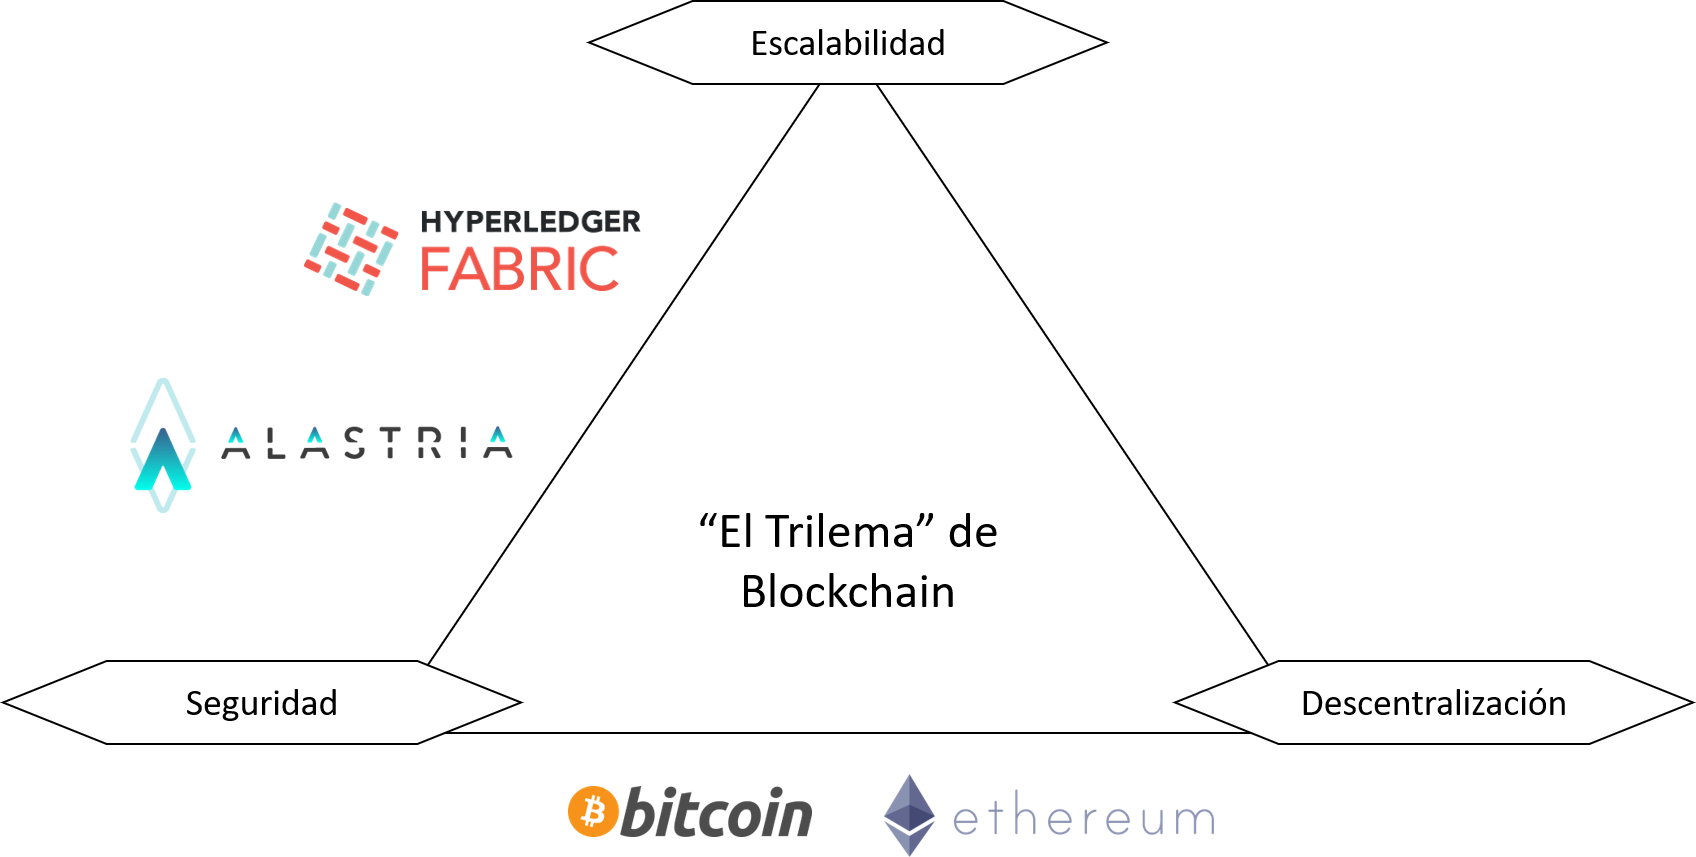
\includegraphics[width=1\textwidth]{imagenes/trilemma2.PNG}
	\caption{\label{fig1}El Trilema de Blockchain. XXX}
\end{figure}

Las redes blockchain tienes 3 aspectos fundamentales a tener en cuenta: seguridad, descentralización y escalabilidad. El problema se denomina trilema porque los protocolos blockchain desarrollados hasta el momento sólo son capaces de ofrecer 2 de estos aspectos poniendo en compromiso al restante. Redes blockchain públicas como la de Bitcoin o Ethereum ofrecen seguridad y descentralización a costa de no ser sistemas escalables. Redes blockchain permisionadas como las de IBM o Alastria ofrecen escalabilidad y seguridad a costa de la descentralización (ya que sólo ciertos nodos elegidos incluyen bloques a la cadena).
Actualmente no existe ningún protocolo blockchain que no comprometa alguno de estos aspectos clave. Conseguir solucionar el problema de la descentralización en las redes permisionadas es imposible por definición. Así que los mayores esfuerzos se centran en atajar el problema de la escalabilidad en redes públicas para intentar solucionarlo o al menos mejorar el rendimiento lo máximo posible.



\section{ARM TrustZone}

Los dispositivos embebidos cada vez manejan datos más sensibles o de más valor. Un claro ejemplo de esto son los dispositivos que manejan datos de cuentas bancarias como contraseñas. A menudo estos dispositivos cumplen otros propósitos, por lo que tienen la capacidad de descargar otro software de terceros. Esto hace que estos dispositivos se encuentren en una posición muy vulnerable. Cuanto más valioso sea el resultado de un ataque realizado con éxito a estos dispositivos, más vulnerables serán, ya que los atacantes estarán dispuestos a emplear mayor tiempo y dinero en realizar un ataque. \newline

El objetivo de la tecnología ARM Trustzone consiste en conseguir que un dispositivo con sistema operativo completo sea a su vez robusto y seguro. Un sistema cuyo diseño de arquitectura hardware y software seguro sea el apropiado, podrá garantizar el correcto uso de datos sensibles. Para conseguir esto hardware y software deben diseñarse para trabajar en sintonía. Los dispositivos identificados como más seguros son aquellos que contienen medidas de seguridad desde su diseño y fabricación. Varias consideraciones de seguridad hardware solamente se podrán incluir en estas fases, añadirlas después será imposible. \newline

La tecnología TrustZone de ARM integra varias medidas de seguridad en procesadores, buses y periféricos. Esto permitirá una gran variedad de posibilidades de arquitecturas seguras en sus dispositivos.


\begin{figure}
	\centering
	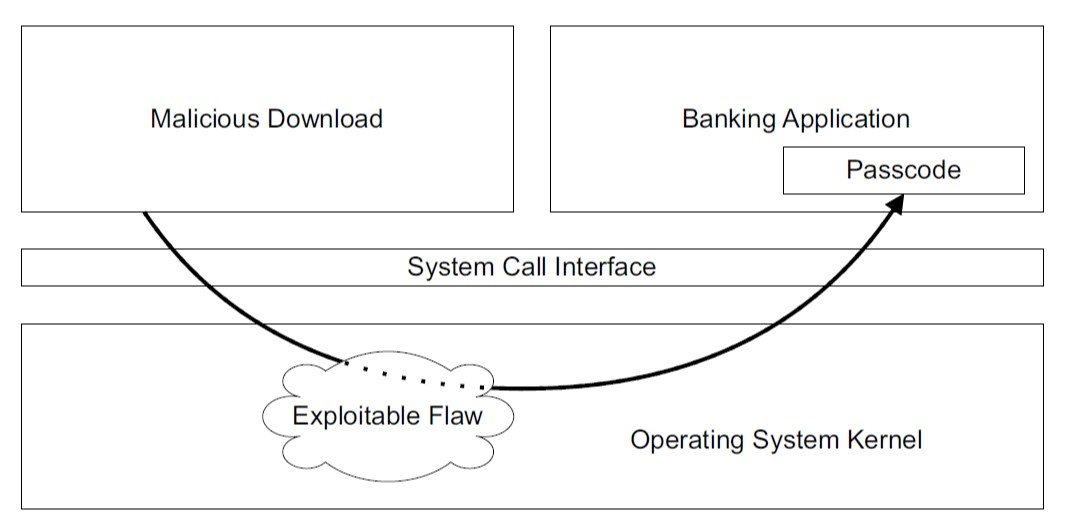
\includegraphics[width=1\textwidth]{imagenes/ataque.jpg}
	\caption{\label{fig1}Escenario de ataque típico en hardware embebido \cite{trustzone}.}
\end{figure}

\subsection{Vectores de ataque}
Para poder estructurar una buena defensa es necesario conocer los distintos tipos de ataque que se pueden llevar a cabo.

\subsubsection{Ataques Hack}
En este tipo de ataque, el atacante solamente es capaz de ejecutar un ataque software. Engloba todo tipo de virus y malware que es descargado e instalado en el dispositivo.

\subsubsection{Ataques Shack}
En este tipo de ataque, el atacante suele tener acceso físico al dispositivo y dispone de un equipamiento muy básico para llevar a cabo el ataque. Con este equipamiento podrá conectarse al dispositivo vía JTAG, escanear los periféricos de entrada y salida, y mediante analizadores de red inspeccionar buses, pines y señales del sistema. A su vez podrán reprogramar espacios de memoria, reemplazar componentes del hardware, forzar buses o pines a estar en alta o baja tensión, etc.

\subsubsection{Ataques de laboratorio}
Es el tipo de ataque más invasivo, ya que el atacante dispone de equipamiento de laboratorio con el que puede llevar a cabo ingeniería inversa sobre el dispositivo. Defenderse de este tipo de ataques no suele ser la estrategia más óptima. Será mucho más óptimo limitar el daño que se pueda ocasionar una vez que el dispositivo a sufrido con éxito uno de estos ataques. El objetivo consiste en hacer el ataque de laboratorio lo menos rentable posible.

\subsection{Seguridad en sistemas embebidos}
Los sistemas embebidos presentan diversas dificultades a la hora de hablar de seguridad. Numerosos procesadores, buses, periféricos, espacios de memoria, etc que complican la seguridad del dispositivo. La solución que haga seguro el dispositivo debe integrar todos estos componentes, ya que no será óptimo hacer seguro cada componente por separado. \newline

Existen diversas soluciones en el mercado encargadas de la seguridad de estos dispositivos.

\subsubsection{Módulos hardware externos de seguridad}
Una de las soluciones de seguridad más extendida para este tipo de dispositivos consiste en integrar un módulo externo al dispositivo en el que se confíe. Un claro ejemplo de estos son las tarjetas SIM.

\subsubsection{Módulos hardware internos de seguridad}
Se trata de módulos dedicados a la seguridad del dispositivo que están integrados en el mismo. En muchos escenarios este tipo de módulos resultan más convenientes. Los ejemplos más representativos de este tipo de módulos son (1) módulos que manejan las operaciones y el almacenamiento de las tareas criptográficas y (2) módulos de procesamiento de tareas sensibles.

\subsubsection{Virtualización software}
La virtualización software es un mecanismo de seguridad en el que una capa de gestión, conocida como hypervisor, separa varias plataformas software independientes. Esta separación se consigue haciendo uso del Memory Management Unit (MMU). Permite que cada uno de los softwares, que corren independientes a los demás, tengan la seguridad de no poder ser atacados por software que esté separado de este.


\subsection{Seguridad TrustZone}

Los principales problemas que surgen con las soluciones que existen actualmente en el mercado se deben principalmente a que estos protegen un determinado componente, dato sensible o activo, pero ignorando un gran abanico de posibilidades de ataque. Esto provoca que en ocasiones se proteja lo que no se debe, o que la protección carezca de sentido. Por ejemplo, no tiene sentido proteger el módulo que gestiona y almacena las claves de criptografía si posteriormente los datos descifrados pueden ser robados fácilmente por un atacante. Esta es la razón por la que se dice que el diseño de la seguridad debe integrar el dispositivo al completo y no solamente sus componentes por separado. \newline

La seguridad de TrustZone se basa en el concepto de una plataforma segura y confiable, una arquitectura hardware que extiende las funcionalidades de seguridad partiendo desde su diseño y fabricación. Si a esto se le suman ciertas metodologías y protocolos de seguridad como Secure Boot o autenticación, se mitigan gran parte de los ataques Shack y Hack. Todo esto en combinación con métodos que intentan mitigar ciertos ataques de laboratorio hacen que se tenga una solución robusta para la seguridad del dispositivo.

\subsubsection{Arquitectura hardware}
El objetivo de TrustZone consiste en proporcionar una arquitectura hardware que permita que el dispositivo se ajuste a los requerimientos de seguridad de cada proyecto en lugar de aportar una solución basada en la idea de “una misma solución sirve para todo”. \newline

En primer lugar, esto se consigue creando un entorno de programación que garantice la confidencialidad y la integridad de todos los datos sensibles y los proteja de la gran mayoría de posibles ataques. Para ello, se realiza un particionado de la arquitectura hardware y software en dos entornos (o mundos como se llamarán a partir de ahora), un Mundo Seguro (MS) y un Mundo Normal (MN). En el Mundo Seguro se realizará todo lo que incumba tareas o datos sensibles y en el Mundo Normal todo lo demás. La lógica hardware presente en el bus AMBA3 AXI será la encargada de hacer que ningún recurso del MS sea accedido por ningún componente del MN, creando un perímetro de seguridad. \newline

Otro aspecto clave de TrustZone es la extensión que se le ha dado a los procesadores ARM. Un único procesador podrá ejecutar código tanto del MS como del MN. Esto elimina la necesidad de tener un procesador que se encargue de las tareas del MS y otro para el MN. Esta característica hará al dispositivo más eficiente. 
Para conseguir esta separación en dos mundos, se han hecho varios cambios en algunos de los componentes de los dispositivos.


\paragraph{Bus AMBA3 AXI}
A cada uno de los buses del sistema se le ha añadido una nueva señal de control tanto en los canales de lectura como en los de escritura. Estos bits, añadidos a la especificación del protocolo del bus AMBA3 AXI, se denominan bits No-Seguros.
\begin{itemize}
	\item AWPROT[1]: Escritura (baja es Segura y alta es No Segura).
	\item ARPROT[1]: Lectura (baja es Segura y alta es No Segura).
\end{itemize}

Todos los buses máster enviarán esta señal cuando se quiera realizar una acción de lectura o escritura, y la lógica de los buses o esclavos debe decodificarlas e interpretarlas correctamente para asegurar que esa separación de mundos no se viola.

\paragraph{Bus periférico AMBA3 APB}

Otra de las principales características de la arquitectura TrustZone consiste en la posibilidad de hacer seguros a los periféricos (controladores de interrupciones, temporizadores y dispositivos de Entrada/Salida). Esto permite una seguridad punto a punto en lugar de únicamente proporcionar una seguridad en el procesado de los datos.

\paragraph{Memoria}

La inclusión del bit No-Seguro al bus se puede ver como una partición en dos de la memoria. El bit No-Seguro se considera como un 33º bit en el espacio de direcciones físicas. Se tendrá por tanto un espacio de direcciones físicas de 32 bits para las transacciones seguras y un espacio equivalente de 32 bits para las no seguras. Se debe tener especial cuidado para asegurar la integridad y coherencia de los datos en todas las localizaciones en las que se almacenen.

\subsubsection{Arquitectura del procesador}
Cada uno de los procesadores físicos provee al sistema de dos procesadores virtuales, uno considerado Seguro y otro No Seguro. Además, también proporciona un mecanismo para cambiar el contexto de ejecución de manera robusta entre Seguro y No Seguro, se le denomina Modo Monitor. Dependiendo de la identidad del procesador virtual desde el que se envíe una transacción, esta será etiquetada como segura o no segura haciendo uso del bit No-Seguro. Esto facilitará la integración de los procesadores virtuales en el sistema. El procesador virtual No Seguro solamente podrá acceder a los recursos del sistema que sean no seguros. En cambio, el procesador virtual Seguro podrá acceder a todos los recursos del sistema. \newline


\begin{figure}
	\centering
	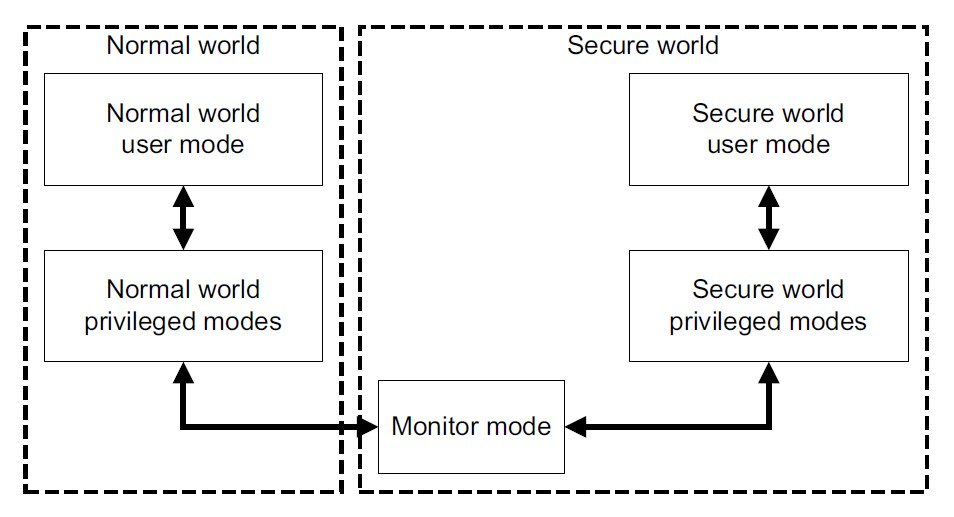
\includegraphics[width=1\textwidth]{imagenes/monitor.jpg}
	\caption{\label{fig1}Estructura de un procesador físico TrustZone \cite{trustzone}.}
\end{figure}


Los mecanismos por los cuales el procesador físico entra en modo monitor son vistos como excepciones al software del modo monitor. La entrada al modo monitor puede estar provocada por el software que ejecuta una determinada instrucción (llamada Secure Monitor Call, SMC) o por mecanismos de excepción hardware (IRQ, FIQ, …). \newline

El mundo en el que el procesador se encuentra está marcado por el bit No-Seguro en el registro Secure Configuration Register (SCR) en CP15. Cuando se encuentra en modo monitor está siempre en el MS.
Se ha mencionado que los espacios de memoria quedan divididos de manera que la memoria está separada para los dos mundos. Esta división que ocurre en la memoria fuera del procesador, debe ocurrir también en los componentes de memoria internos al procesador como es el sistema de memoria L1. El principal componente de la memoria L1 es el Memory Management Unit (MMU). El MMU es capaz de mapear el espacio de direcciones de memoria virtual que es visto por el software ejecutándose en el procesador con el espacio de direcciones físico existente fuera del procesador. La traducción se realiza haciendo uso de una tabla de traducción controlada por software.
En un procesador con TrustZone, el hardware proporciona dos MMUs, una para cada procesador virtual. Esto permite que cada mundo posea su propia tabla de traducción de direcciones de manear totalmente independiente.

\subsubsection{Arquitectura software}

La implementación de un Mundo Seguro en el dispositivo requiere de un software seguro que se ejecute y haga uso de los datos sensibles que se encuentren en este. Cada desarrollador puede crear un MS que se adecúe a las necesidades y requerimientos de su sistema. \newline

Existen muchas posibles arquitecturas software que podrán ser desarrolladas en el Mundo Seguro de un procesador con TrustZone habilitado. La arquitectura más compleja que se puede alojar en un MS es un sistema operativo. La más sencilla es una librería de código alojada en el MS. Entre estos dos extremos existen un gran abanico de posibilidades intermedias.


\paragraph{Sistema operativo} 
Un sistema operativo dedicado en el MS es un diseño complejo pero que abre un gran abanico de posibilidades. Puede simular la ejecución concurrente de varias aplicaciones del MS, descargar nuevas aplicaciones seguras y otro tipo de tareas seguras que serán totalmente independientes del MN. Cada procesador virtual tendrá un sistema operativo completo y se comportará como tal.

\begin{figure}
	\centering
	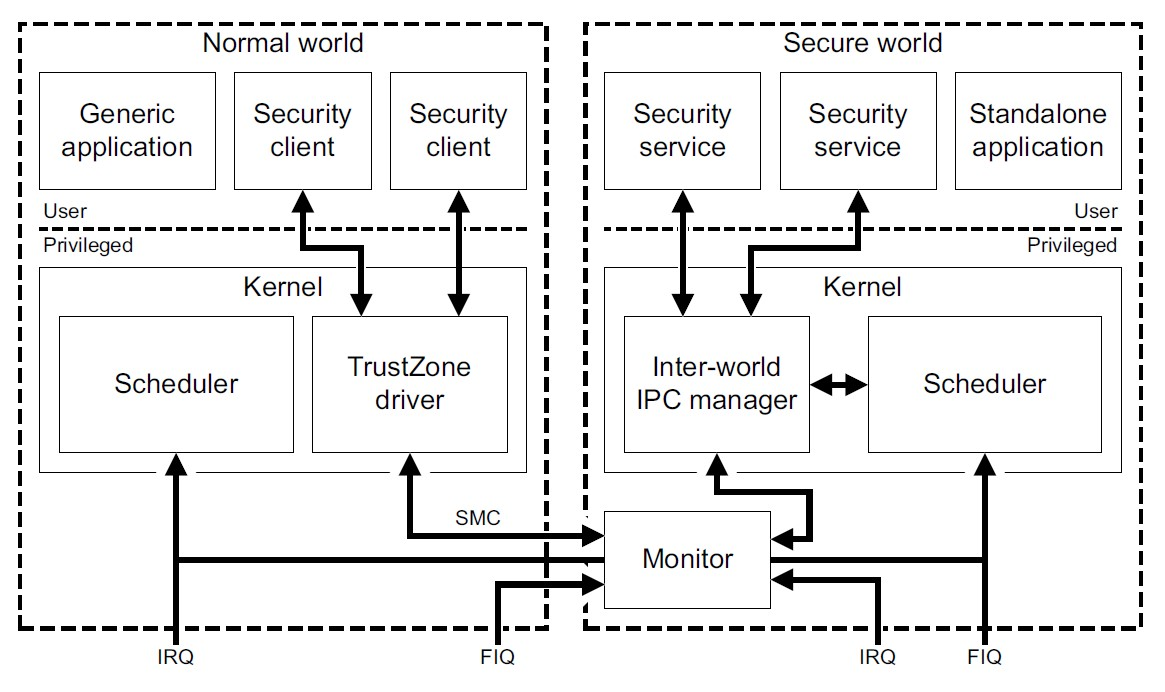
\includegraphics[width=1\textwidth]{imagenes/secureSO.jpg}
	\caption{\label{fig1}Esquema de un SO sobre el Mundo Seguro \cite{trustzone}.}
\end{figure}

\paragraph{Librería de código}
Muchos casos de uso no justificarán la complejidad de un sistema operativo en el MS ya que sus requerimientos son mucho menores. Una sencilla librería de código que ejecute una tarea en el MS puede ser suficiente para muchos casos de uso. Esta librería se ejecutará mediante las pertinentes llamadas realizadas desde el sistema operativo del MN. El MS es por tanto un esclavo del MN ya que el MS no se podrá ejecutar independientemente.

\subsubsection{Arrancado de un sistema seguro}
Uno de los puntos más críticos de un sistema seguro es el arrancado. Muchos de los ataques se centran en la modificación del sistema cuando este se encuentra apagado. Por ejemplo, reemplazar la imagen del MS que se encuentra en la memoria flash del dispositivo con una imagen del MS modificada. Por tanto, para que el sistema no sea vulnerable se deberá comprobar la autenticidad del código en el tiempo de arranque. La estrategia que se sigue consiste en una cadena de confianza para el software del mundo seguro que partirá de un punto difícilmente manipulable. Esto se corresponderá con una determinada secuencia de arrancado.

\paragraph{Secuencia de arrancado}
Cuando el dispositivo se enciende, un procesador con TrustZone habilitado siempre comienza en el Mundo Seguro. Esto permite que se puedan realizar diversas comprobaciones de seguridad antes de que el Mundo Seguro arranque y tenga alguna oportunidad de modificar algún aspecto del sistema.\newline

La figura XXXXXXXXXXXXx muestra una típica secuencia de arrancado. Tras encender el dispositivo se suele ejecutar un código que se encuentra en la ROM del dispositivo y que será el encargado de inicializar periféricos críticos del dispositivo. Este da paso a un código de arranque de segundo nivel que se encuentra en la memoria no-volátil externa del dispositivo. La secuencia continuará avanzando hasta que se haya completado el arranque del Mundo Seguro. Posteriormente se da paso al Mundo Normal y una vez este se haya completado se puede decir que el sistema se está ejecutando correctamente.
Para que esta secuencia tenga sentido se deben añadir comprobaciones criptográficas en cada fase del arrancado seguro. Cada fase de la secuencia realizará una comprobación de la integridad de la siguiente fase a ejecutar. Se previene así que arranque cualquier tipo de código malicioso no autorizado o modificado. \newline

\begin{figure}
	\centering
	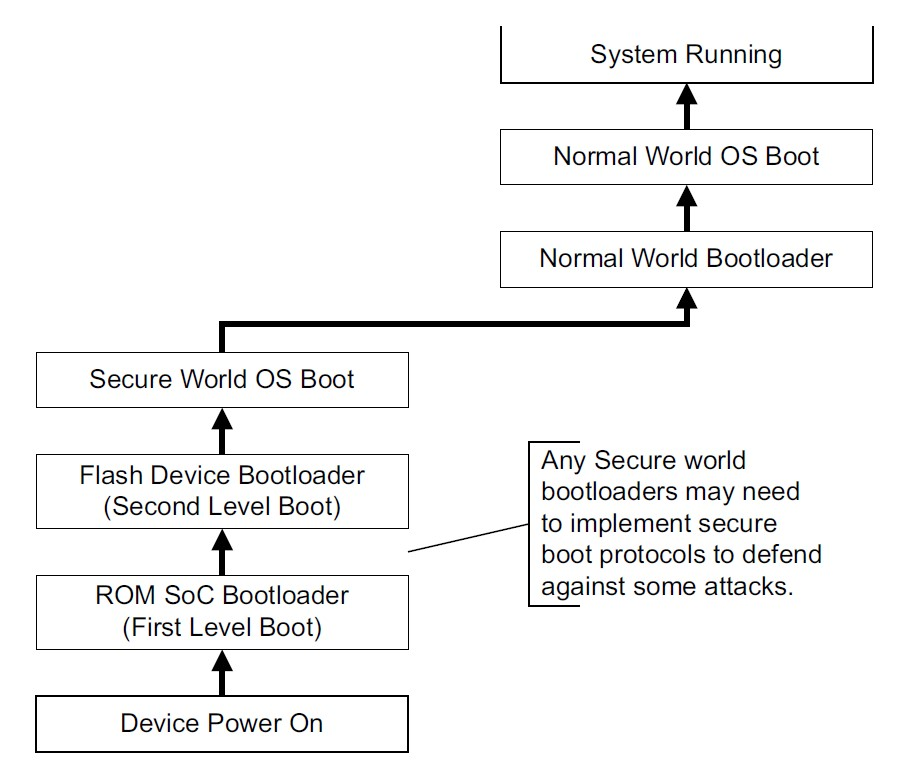
\includegraphics[width=1\textwidth]{imagenes/secureboot.jpg}
	\caption{\label{fig1}Secuencia de arrancado seguro \cite{trustzone}.}
\end{figure}

Para esta tarea se utiliza un algoritmo de cifrado de clave asimétrica, RSA-PSS (Rivest, Shamir and Adleman – Probabilistic Signature Scheme). En este protocolo, un vendedor de confianza generará una firma del código que se quiere desplegar haciendo uso de su clave privada. Esta firma irá incluida en el binario del software. La clave pública del vendedor se almacenará en el dispositivo en alguno de sus registros dedicados a este propósito que no podrán ser alterados. Esta clave pública se utilizará para verificar que el binario proporcionado por el vendedor no ha sido modificado, por ello se necesita que esta clave pública no pueda ser modificada por una propiedad de un atacante.
Se crea por tanto una cadena de confianza que nace en un componente del dispositivo en el que se confía. A partir de este se podrá autenticar cualquier otro componente o software antes de que sea ejecutado. Una vez que se ha ejecutado la autenticación de la primera fase de la secuencia, las próximas autenticaciones de la secuencia podrán ser realizadas con claves públicas diferentes. Solamente la autenticación de la primera fase debe realizarse con la clave que se encuentra en los registros One-Time-Programmable (OTP) del dispositivo.




